\section{Basics}

\subsection{Digital Signal Processing}

\subsubsection{Sampling and quantization}

If data from the real world should be processed in a digital system, it has to be sampled.
This process is has significant effects on the original signal so they have to be considered if
\ac{DSP} is taken seriously.

\subsubsection{Digital Filters}

\subsubsubsection{Finite Impulse Response Filter}

Digital Filters are a huge field of digital signal processing. The most common filters are \ac{FIR}-filters.
The basic structure is a weighted shift register without feedback. The missing feedback is what makes
the \ac{FIR}-filter stable per construction.

In \autoref{fig:FIR-filter} the structure of a \ac{FIR}-filter is shown.

\begin{figure}[!h]
    \centering
    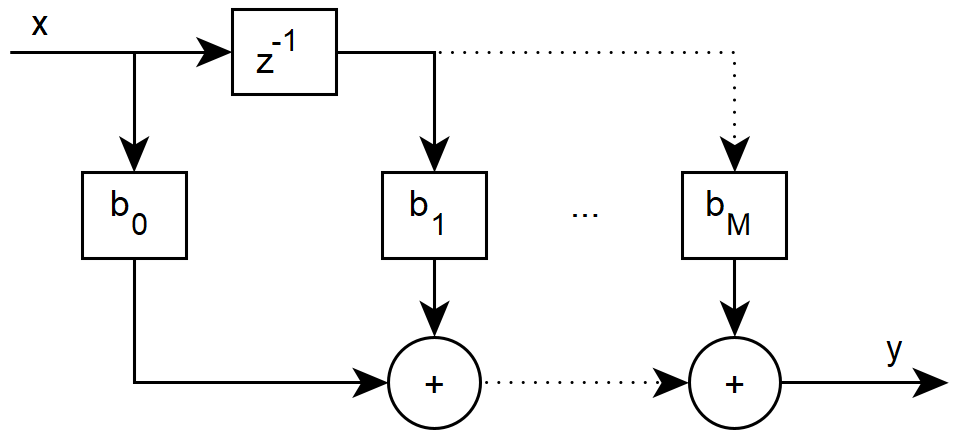
\includegraphics[width=7cm]{img/fir.png}
    \caption{Basic structure of a $M$ order \ac{FIR}-filter in the first canonical form \cite{meyer_signalverarbeitung}}
    \label{fig:FIR-filter}
\end{figure}

It can be seen that there are multiple components in this filter. The first component is the delay block,
which is described as $z^{-1}$. This block is responsible for adding a delay of one clock cycle to the input data.
Secondly, there are multiplikation blocks, noted as $b_M$. These blocks weight the input data and give the
result to an adder, which adds $M+1$ weighted and delayed signal samples. This sum is the output of an
\ac{FIR}-filter. It should be mentioned that the signal is transmitted without delay weighted with the coefficient
$b_0$.

The input signal is $x$, whereas the output is $y$. The order of this Filter is $M$ which means the amount of
filter taps or delay blocks.

A special case of the \ac{FIR}-filter is the \textit{Moving Average Filter}, at which all coefficients are $\frac{1}{M+1}$.

The whole system can be described with the difference equation in the time-domain (\autoref{eq:fir-difference-eq})

\begin{equation}
    y[n] = b_0 \cdot x[n] + b_1 \cdot x[n-1] + ... + b_M \cdot x[n-M]
    \label{eq:fir-difference-eq}
\end{equation},

or with the transfer function in the z-domain (\autoref{eq:fir-transfer-func})

\begin{equation}
    H(z) = b_0 + b_1 \cdot z^{-1} + ... + b_M \cdot z^{-M}
    \label{eq:fir-transfer-func}
\end{equation}.

The output can be calculated with the convolution (noted as $*$) of the impulse response $h[n]$, which is simply the
union of the filter coefficients, and the input signal $x[n]$ (\autoref{eq:conv}).

\begin{equation}
    y[n] = x[n] * h[n]
    \label{eq:conv}
\end{equation}

Another way to describe the filterung result is in the frequency domain.
If the frequency of the input is given with $X(z)$ and the frequency response of the filter is $H(z)$
then the ouput is $Y(z)$ which can be calculated like shown in \autoref{eq:freq-response}.

\begin{equation}
    Y(z) = X(z) \cdot H(z)
    \label{eq:freq-response}
\end{equation}

The stability of the \ac{FIR}-filter is characteristic, this can be seen in the pole-zero plane. All poles are in
the middle of the unit cyrcle, which is necessary for the stability of a system.

If the value of the z-plane is evaluated on the unit cyrcle the result is the frequency response of the filter
(\autoref{fig:FIR-z-plane-and-freq}).

\begin{figure}[!h]
    \begin{subfigure}[c]{0.35\textwidth}
        \centering
        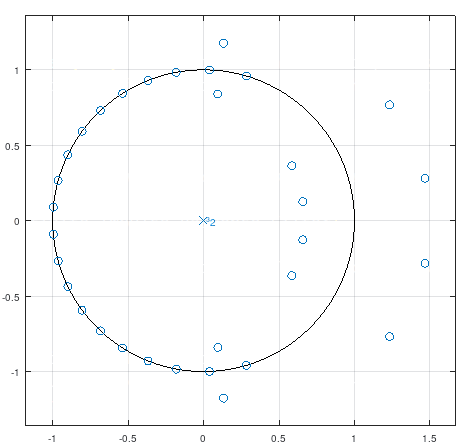
\includegraphics[width=\textwidth]{img/fir-zplane.png}
    \end{subfigure}
    \begin{subfigure}[c]{0.65\textwidth}
        \centering
        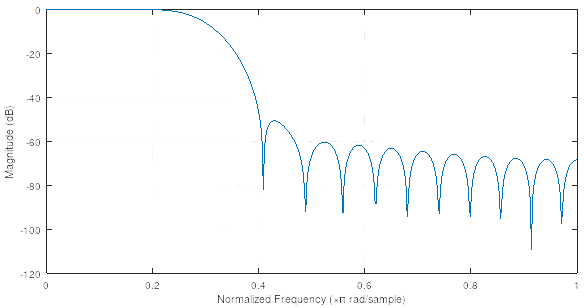
\includegraphics[width=\textwidth]{img/fir-freq.png}
    \end{subfigure}
    \caption{z-plane plot (left) and frequency response (right) of a \ac{FIR}-filter}
    \label{fig:FIR-z-plane-and-freq}
\end{figure}

%% //TODO: pole zero plane, calculation of coeffs, output (conv in time, mult. in z-domain)?

\subsubsubsection{Infinite Impulse Response Filter}

Another Filter type is the \ac{IIR} filter. The structure is fully recursive as it is shown in \autoref{fig:IIR-filter}.

\begin{figure}[!h]
    \centering
    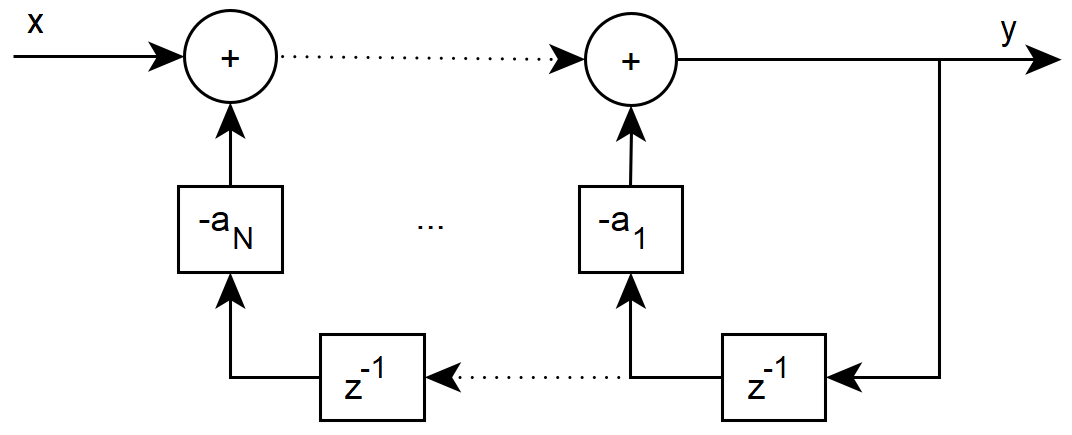
\includegraphics[width=7cm]{img/iir.png}
    \caption{Basic structure of a $M$ order \ac{IIR}-filter in the first canonical form \cite{meyer_signalverarbeitung}}
    \label{fig:IIR-filter}
\end{figure}

\subsection{Audio-Interfaces}

\subsubsection{Inter-Integrated Sound}

The \ac{I2S} protocol was developed by \textit{Philips} to share audio between \acp{IC}.
A similarity to the \ac{SPI} protocol can be recognized.

There are three signal lines:
\begin{itemize}
    \item SCK: Clock signal
    \item SD: Data signal
    \item WS: Word select, for ditinction between left and right channel
\end{itemize}
So the data is transmitted over the same signal line by time division multiplexing. 
To illsutrate the timing of the protocol the corresponding diagrams are shown in \autoref{fig:i2s-timing} \cite{nxp_i2s}.

\begin{figure}[!h]
    \centering
    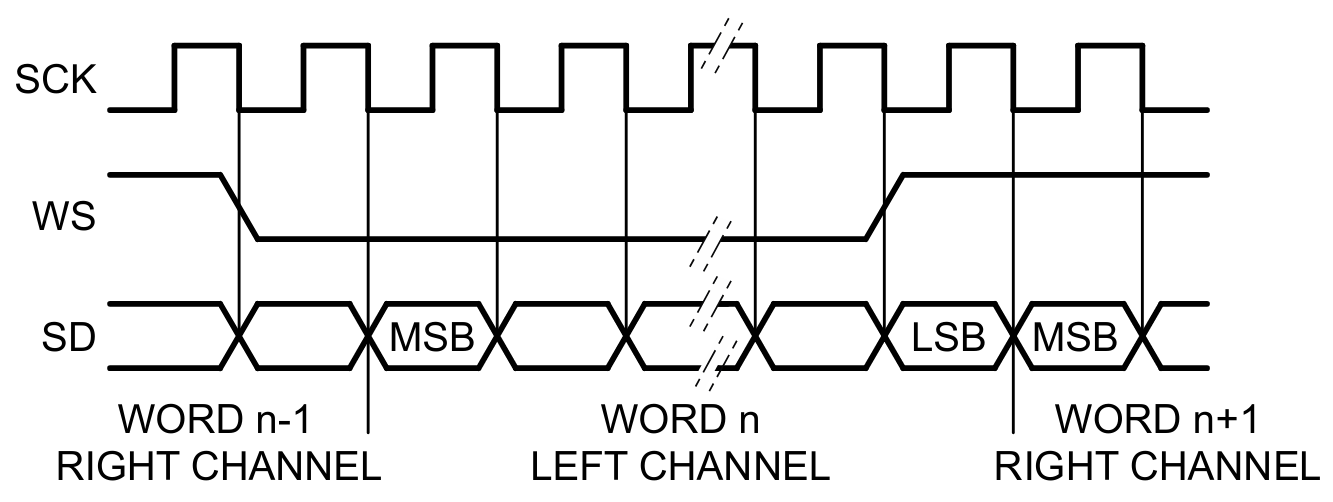
\includegraphics[width=10cm]{img/i2s_timing.png}
    \caption{Timing diagramm of the \ac{I2S} protocol \cite{nxp_i2s}}
    \label{fig:i2s-timing}
\end{figure}

The word length can vary between transmitter and receiver. That is why the \ac{MSB} is sent first in the standard 
configuration. Additionally the participants do not need to know the word length of the counterpart \cite{nxp_i2s}.

The wiring of this serial bus is possible in three basic configurations (shown in \autoref{fig:i2s-config}).
Thereby the master is always responsible for the SCK and the WS line.

\begin{figure}[!h]
    \centering
    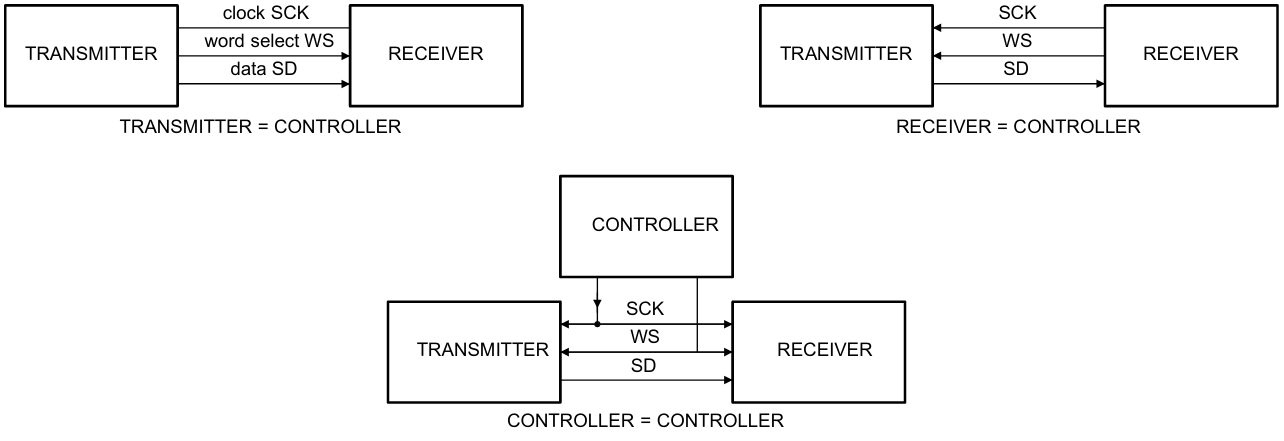
\includegraphics[width=14cm]{img/i2s_config.png}
    \caption{The three basic configurations of the \ac{I2S} protocol \cite{nxp_i2s}}
    \label{fig:i2s-config}
\end{figure}

%%// TODO: DMA
